\subsection{Ampliación de capacidad}
Para ampliar la capacidad de una memoria, se deben agregar chips de memoria en serie y se deben conectar las líneas de dirección de manera que se seleccione el chip adecuado.

\subsubsection{Ejemplo}
En el ejemplo se debe conformar un banco de
4K direcciones, cada una de 4 bits, y para hacerlo se cuenta con chips de 1K x 4 bits. En primer lugar dividimos la capacidad total de memoria necesaria por la capacidad de cada chip, a los efectos de obtener la cantidad de chips que debemos emplear. En este caso se necesitarán 4 chips.

Se pretende aumentar la cantidad de direcciones disponibles. Cada chip posee 10 líneas de dirección, pero el banco es de 4K, o sea que necesita 12 líneas. Las líneas A0, hasta A9 (10 bits) van a todos los chips simultáneamente. Las líneas restantes (A10 y A11) entran a un decodificador cuya función es la de ir habilitando uno a uno, a los diferentes chips de memorias del banco, con el objeto de evitar un conflicto en el Bus de Datos. De este modo, sólo un chip por vez estará activo, quedando el resto, en alta impedancia, con lo que cada chip pondrá, o recibirá, datos del bus de datos en forma individual.

Lo vamos a representar con una tabla, primero tendremos el chip, cada chip tiene las direcciones que tomará, y luego las líneas de dirección que se le asignan. Podemos notar que como se busca tener 4K direcciones, se necesitan 12 líneas de dirección.

\begin{figure}[h]
    \centering
    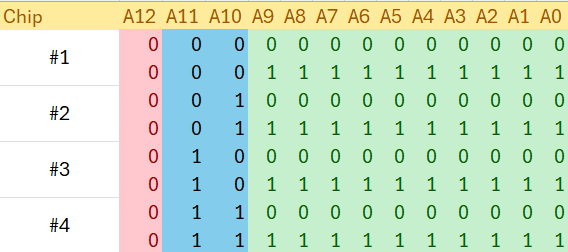
\includegraphics[scale=0.8]{img/tabla.png}
\end{figure}
Se puede observar que el banco funcionará siempre que A12 sea 0, ya que en caso contrario se generarían espejos. Luego la parte verde son las líneas de dirección que comparten todos los chips, y la parte azul son las líneas de dirección que se le asignan a cada chip. Es decir las que usaremos para seleccionar el chip que queremos leer o escribir. Para ello podemos notar que usar un decodificador de 2x4 nos permitirá seleccionar el chip que queremos leer o escribir.

\begin{figure}[h]
    \centering
    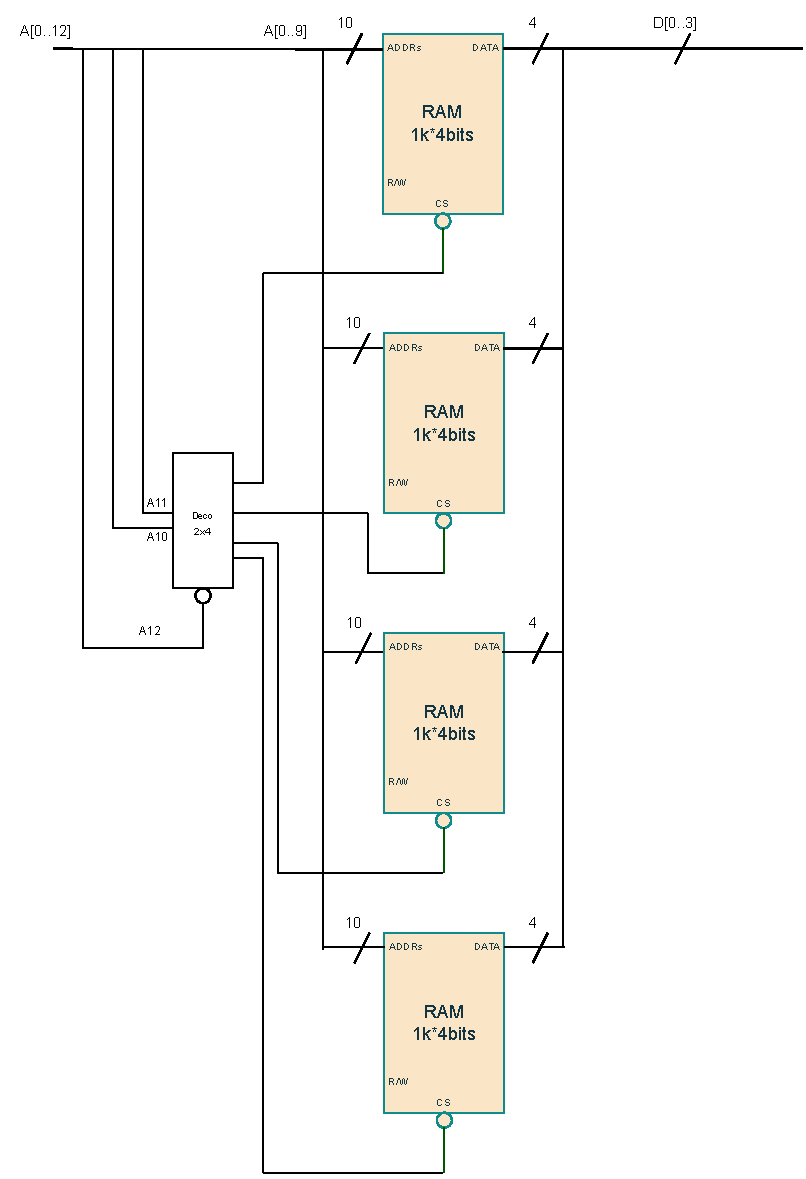
\includegraphics[scale=0.8]{img/ejmemorias.pdf}
\end{figure}